\newglossaryentry{psd}
{name={positive semi-definite (psd)},
	description={A\index{positive semi-definite (psd)} (real-valued) 
	             symmetric \gls{matrix} $\mQ = \mQ\,^{T} \in \mathbb{R}^{\featuredim \times \featuredim}$ 
	 	         is referred to as psd if $\featurevec\,^{T} \mQ \featurevec \geq 0$ 
				 for every \gls{vector} $\featurevec \in \mathbb{R}^{\featuredim}$. 
	 	         The property of being psd can be extended from \glspl{matrix} to (real-valued) 
	 	         symmetric \gls{kernel} \glspl{map} $\kernel: \featurespace \times \featurespace \rightarrow \mathbb{R}$ 
	 	         (with $\kernel(\featurevec,\featurevec') = \kernel(\featurevec',\featurevec)$)
	 	         as follows: For any finite set of \glspl{featurevec} $\featurevec^{(1)}, \,\ldots, \,\featurevec^{(\samplesize)}$, 
	 	         the resulting \gls{matrix} $\mQ \in \mathbb{R}^{\samplesize \times \samplesize}$ with 
		        entries $Q_{\sampleidx,\sampleidx'} = \kernelmap{\featurevec^{(\sampleidx)}}{\featurevec^{(\sampleidx')}}$ 
		        is psd \cite{LearningKernelsBook}.
			\\
		See also: \gls{matrix}, \gls{kernel}.},
	first={positive semi-definite (psd)},
	type=math, 
	text={psd}  
}

\newglossaryentry{normalmatrix}
{name={normal matrix},
	description={A square matrix $\mA \in \mathbb{C}^{\nrfeatures \times \nrfeatures}$ 
                 that commutes with its conjugate transpose, i.e., $\mA\mA^{H}=\mA^{H}\mA$. 
                 Normal matrices admit an orthonormal basis of \glspl{eigenvector} and are 
                 unitarily \gls{diagonalizable}.},
	first={normal matrix},
    type=math, 
	plural={normal matrices},
	firstplural={normal matrices},
	text={normal matrix}
}

\newglossaryentry{spectraldecomp}
{name={spectral decomposition},
	description={Every \gls{normalmatrix} $\mA \in \mathbb{C}^{\nrfeatures \times \nrfeatures}$ 
                 admits\index{spectral decomposition} a spectral decomposition of the form \cite{HornMatAnalysis,Axler2025}
       \begin{align}
        \nonumber
            \mA 
            % & = 
            % \big[ \vu^{(1)}\ \cdots\ \vu^{(\nrfeatures)}\big]
            % \pmatrix{
            % \eigval{1} &        &        & 0\\
            %         & \eigval{2} &     &  \\
            %         &        & \ddots &  \\
            % 0         &        &        & \eigval{\nrfeatures}
            % }
            % \pmatrix{
            % \big(\vu^{(1)}\big)^{H}\\
            % \vdots\\
            % \big(\vu^{(\nrfeatures)}\big)^{H}
            % } \nonumber \\
                & = \sum_{\featureidx=1}^{\nrfeatures} \eigval{\featureidx} \vu^{(\featureidx)} \big(\vu^{(\featureidx)})^{H} \nonumber \\ 
       \end{align}
      with an orthonormal basis $\vu^{(1)},\ldots,\vu^{(\nrfeatures)}$. 
       \begin{figure}[t]
            \centering
            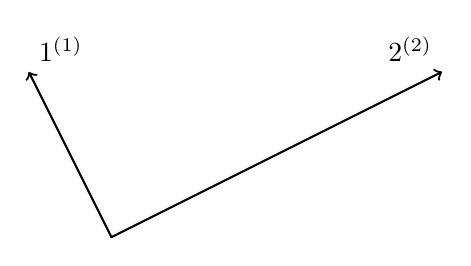
\begin{tikzpicture}[scale=2.1, line cap=round, line join=round]
            % two eigenvectors with different lengths
            \draw[->, thick] (0,0) -- (-0.5,1) node[above right] {$\eigval{1} \vu^{(1)}$};
            \draw[->, thick] (0,0) -- (2.0,1) node[above left]  {$\eigval{2} \vu^{(2)}$};
            \end{tikzpicture}
            \caption{The spectral decomposition of a \gls{normalmatrix} $\mA$ provides 
                     an orthonormal basis $\vu^{(1)}, \vu^{(2)}$. Applying $\mA$ 
                     amounts to a scaling of the basis \glspl{vector} by the 
                     \glspl{eigenvalue} $\eigval{1},\eigval{2}$.\label{fig:eigenvectors-length_dict}}
            \end{figure}
       Each basis element $\vu^{(\featureidx)}$ 
       is an \gls{eigenvector} of $\mA$ with corresponding \gls{eigenvalue} $\eigval{\featureidx}$, 
       for $\featureidx=1,\ldots,\nrfeatures$.
       },
	first={spectral decomposition},
    type=math,
	text={spectral decomposition}
}


\newglossaryentry{symmetricmatrix}
{name={symmetric matrix},
	description={A square\index{symmetric matrix} \gls{matrix} $\mA$ with real-valued 
                 entries that is equal to its transpose, i.e., $\mA=\mA^{T}$. Every 
                 symmetric \gls{matrix} is a \gls{normalmatrix}.},
	first={symmetric matrix},
	plural={symmetric matrices},
    type=math,
	firstplural={symmetric matrices},
	text={symmetric matrix}
}

% \newglossaryentry{transpose}
% {name={transpose},
% 	description={The transpose\index{transpose} of a \gls{matrix} is obtained by exchanging 
%                  rows and columns. For a matrix $\mA$, its transpose is denoted 
%                  $\mA^{T}$ and satisfies $(\mA^{T})_{i,j}=\mA_{j,i}$.},
% 	first={transpose},
%     type=math, 
% 	text={transpose}
% }

% \newglossaryentry{hermitianmatrix}
% {name={Hermitian matrix},
% 	description={A square matrix $\mA \in \mathbb{C}^{\nrfeatures \times \nrfeatures}$ 
%                  that coincides with its conjugate transpose, i.e., $\mA=\mA^{H}$. 
%                  Trivally, a Hermitian matrix is also a \gls{normalmatrix}.},
% 	first={Hermitian matrix},
%     type=math, 
% 	plural={Hermitian matrices},
% 	firstplural={Hermitian matrices},
% 	text={Hermitian matrix}
% }

\newglossaryentry{dimension}
{name={dimension},
	description={The\index{dimension} dimension $\dim \mathcal{A}$ of a 
		\gls{vectorspace} $\mathcal{A}$ is the cardinality of any 
		\gls{basis} of $\mathcal{A}$ \cite{StrangLinAlg2016}. 
		Strictly speaking, this definition applies only to finite-dimensional \glspl{vectorspace}, 
		i.e., those that possess a finite \gls{basis}. 
		\begin{figure}[H]
			\begin{tikzpicture}[scale=1]
  			% Axes (optional; remove if you want it even more minimal)
  			%	\draw[->, thin, gray] (-0.2,0) -- (3.2,0) node[right] {$\vw^{(1)}$};
  			%	\draw[->, thin, gray] (0,-0.2) -- (0,3.2) node[above] {$\vw^{(1)}$};
  			\coordinate (O) at (0,0);
  			% Basis 1: standard (solid)
  			\draw[->, thick] (O) -- (1.8,0) node[below right] {$\ve^{(1)}$};
  			\draw[->, thick] (O) -- (0,1.6) node[above left] {$\ve^{(2)}$};
  			% Basis 2: rotated by ~45° (dashed)
			\draw[->, thick, dashed, shift={(3.5,0.5)}] (0,0) -- (1.2,1.2) node[above right] {$\vu^{(1)}$};
			\draw[->, thick, dashed, shift={(3.5,0.5)}] (0,0) -- (-1.2,1.2) node[above left] {$\vu^{(2)}$};
  			% Basis 3: non-orthogonal / skewed (dotted)
  			\draw[->, thick, dotted, shift={(-2.5,-2.5)}] (O) -- (2.0,0.6) node[above right] {$\vw^{(1)}$};
  			\draw[->, thick, dotted, shift={(-2.5,-2.5)}] (O) -- (0.4,1.8) node[left] {$\vw^{(2)}$};
  			% Simple legend
 			% \node[anchor=west] at (1.6,-0.6) {\footnotesize \textbf{Bases:} solid = standard,\; 
 			% dashed = rotated,\; dotted = skewed};
			\end{tikzpicture}
		\caption{Three \glspl{basis}, $\big\{\ve^{(1)},\ve^{(2)} \big\}, \big\{\vu^{(1)},\vu^{(2)} \big\},
		\big\{\vw^{(1)},\vw^{(2)} \big\}$, for the \gls{vectorspace} $\mathbb{R}^{2}$.} 
		\end{figure}
		For such spaces, all \glspl{basis} have the same cardinality, which is the dimension of the space 
		\cite[Ch.~2]{Axler2025}.	
   			 \\
		See also: \gls{vectorspace}, \gls{basis}. }, 
	text={dimension}, 
	type=math,
	first={dimension}  
}

\newglossaryentry{linearlyindep}
{name={linearly independent},
	description={A subset $\{\va^{(1)}, \,\ldots, \,\va^{(\nrfeatures)}\} \in \mathcal{V}$ 
		of a \gls{vectorspace} is linearly independent\index{linearly independent} 
		if there is no nontrivial linear combination of these \glspl{vector} that 
		equals the zero \gls{vector} \cite{StrangLinAlg2016}. 
		In other words, $$\sum_{\featureidx=1}^{\nrfeatures} \alpha_{\featureidx} \va^{(\featureidx)} = \mathbf{0}	
		\quad \text{ implies } \quad \alpha_{1} = \alpha_{2} = \ldots = \alpha_{k} = 0.$$ 
			\\ 
		See also: \gls{vectorspace}, \gls{vector}, \gls{dimension}, \gls{basis}.}, 
	text={linearly independent}, 
	type=math,
	first={linearly independent}  
}

\newglossaryentry{basis}
{name={basis},
	description={A basis\index{basis} of a \gls{vectorspace} $\mathcal{V}$ 
		is a set of \gls{linearlyindep} \glspl{vector} $\{\va^{(1)}, \,\ldots, \,\va^{(\nrfeatures)}\}$ such 
		that any \gls{vector} $\va \in \mathcal{A}$ can be expressed as a linear combination 
		of the basis \glspl{vector}, i.e.,	
		$$ \va = \sum_{\featureidx=1}^{\nrfeatures} \alpha_{\featureidx} \va^{(\featureidx)} 
		\quad \text{ for some } \alpha_{1}, \,\ldots, \,\alpha_{\nrfeatures} \in \mathbb{R}. $$
			\\
		See also: \gls{vectorspace}, \gls{linearlyindep}, \gls{vector}. },
	text={basis}, 
	firstplural={bases}, 
	plural={bases}, 
	type=math,
	first={basis} 
}


\newglossaryentry{widematrix}
{name={wide matrix},
 description={A\index{wide matrix} \gls{matrix} 
   		$\mA \in \mathbb{R}^{\samplesize \times \nrfeatures}$ 
		is referred to as wide if it has more columns than rows, i.e., when $\nrfeatures > \samplesize$.
		\\ 
		See also: \gls{matrix}. },
	text={wide matrix}, 
	firstplural={wide matrices}, 
	plural={wide matrices}, 
	type=math,
   	first={wide matrix} 
}

\newglossaryentry{randomexperiment}
{name={random experiment},
	description={A random experiment\index{random experiment} is a physical (or abstract) process 
    	 	that produces an outcome $\outcome$ from a set $\samplespace$ of possibilities. 
	 	This set of all possible outcomes is referred to as the \gls{samplespace} of 
	 	the experiment. The key characteristic of a random experiment is that its 
	 	outcome is unpredictable (or uncertain). Any measurement or observation 
	 	of the outcome is a \gls{rv}, i.e., a \gls{function} of the outcome $\outcome \in \samplespace$. 
	 	\Gls{probability} theory uses a \gls{probspace} as a mathematical structure for the study of 
	 	random experiments. A key conceptual property of a random experiment is that it can 
	 	be repeated under identical conditions. Strictly speaking, repeating a random experiment 
	 	a given number of $\samplesize$ times defines a new random experiment. The outcomes 
	 	of this new experiment are length-$\samplesize$ sequences of outcomes 
	 	from the original experiment (see Fig. \ref{fig_randomexperiment_dict}). While the outcome of a single experiment is 
	 	uncertain, the long-run behaviour of the outcomes of repeated experiments 
	 	tends to become increasingly predictable. This informal claim can be made 
	 	precise via fundamental results of \gls{probability} theory, such as the \gls{lln} 
	 	and the \gls{clt}.
	 	\begin{figure}[H]
		\begin{center}
	 		\begin{tikzpicture}[>=Stealth, node distance=1.5cm and 2cm, every node/.style={font=\small}]
			\node (experiment) [draw, rectangle, rounded corners, minimum width=2.6cm, align=center] {random\\experiment};
			\node (omega) [right=of experiment] {$\outcome \in \samplespace$};
			\coordinate (rightpad) at ($(omega.east) + (0.2,0)$);
			\draw[->] (experiment) -- (omega);
			\node (sequence) [below=of experiment, yshift=-0.5cm] {$(\outcome^{(1)}, \,\outcome^{(2)}, \,\dots, \,\outcome^{(\samplesize)})$};
			\node (sequence1) [below=of sequence, yshift=-0.5cm] {$(\datapoint^{(1)}, \,\datapoint^{(2)}, \,\dots, \,\datapoint^{(\samplesize)})$};
			\draw[->, thick] (experiment.south) -- node[midway, right, xshift=3pt] {repeat $\samplesize$ times} (sequence.north);
			\draw[->, thick] (sequence.south) -- node[midway, right, xshift=3pt] {\glspl{rv}} (sequence1.north);
			% Anchor node ~60% along the repeat arrow
			\path (experiment.south) -- (sequence.north) coordinate[pos=0.6] (repeatpoint);
			% Dotted rounded box enclosing experiment and part of repeat arrow
        			\node[draw=black, rounded corners, dotted, fit={(experiment) (repeatpoint) (rightpad)}, inner sep=8pt, label=above:{new random experiment with $\samplespace' = \samplespace \times \ldots \times \samplespace$}] {};
	 		\end{tikzpicture}
	     	\end{center}
		\caption{A random experiment produces an outcome $\outcome \in \samplespace$ from a set 
		of possibilities (i.e., a \gls{samplespace}) 
		$\samplespace$. Repeating the experiment $\samplesize$ times yields another random 
		experiment, whose outcomes are sequences 
		$(\outcome^{(1)}, \,\outcome^{(2)}, \,\dots, \,\outcome^{(\samplesize)}) \in \samplespace\times\ldots\times \samplespace$. 
		One example of a random experiment arising in many \gls{ml} applications is the gathering 
		of a \gls{trainset} $\datapoint^{(1)},\,\ldots,\,\datapoint^{(\samplesize)}$. \label{fig_randomexperiment_dict}}
	 	\end{figure} 
	 	Examples for random experiments arising in \gls{ml} applications include the following: 
	 	\begin{itemize} 
			\item \Gls{data} collection: The \glspl{datapoint} collected in \gls{erm}-based methods 
			can be interpreted as \glspl{rv}, i.e., as \glspl{function} of the outcome $\outcome \in \samplespace$ 
			of a random experiment. 
			\item \Gls{stochGD} uses a random experiment at each iteration to select a subset of 
			the \gls{trainset}. 
			\item \Gls{privprot} methods use random experiments to perturb  
			the outputs of an \gls{ml} method to ensure \gls{diffpriv}. 
	 	\end{itemize} 
		See also: \gls{samplespace}, \gls{rv}, \gls{probability}, \gls{probspace}.},
 	firstplural={random experiments},
 	plural={random experiments},
	type=math, 
 	first={random experiment},
 	text={random experiment}
}

\newglossaryentry{pseudoinverse}
{name={pseudoinverse},
  description={The \index{pseudoinverse}Moore–Penrose pseudoinverse $\mA^{+}$ 
 	of a \gls{matrix} $\featuremtx \in \mathbb{R}^{\samplesize \times \nrfeatures}$ 
	generalizes the notion of an \gls{inverse} \cite{GolubVanLoanBook}. 
	The pseudoinverse arises naturally in \gls{ridgeregression} for a 
	\gls{dataset} with \gls{featuremtx} $\featuremtx$ and \gls{labelvec} 
	$\labelvec$ \cite[Ch.\ 3]{hastie01statisticallearning}. 
	The \glspl{modelparam} learned by \gls{ridgeregression} 
  	are given by
  	\[
  	\widehat{\weights}^{(\regparam)}  = \big(\featuremtx^{T} \featuremtx + \regparam \mI \big)^{-1} \featuremtx^{T} \vy, \quad \regparam > 0.
  	\]
  	We can then define the pseudoinverse $\featuremtx^{+} \in \mathbb{R}^{\nrfeatures \times \samplesize}$ via 
  	the limit \cite[Ch. 3]{benisrael2003generalized}
  	\[
  	\lim_{\regparam \to 0^+} \widehat{\weights}^{(\regparam)} = \featuremtx^+ \vy.
  	\]
	\\
	See also: \gls{matrix}, \gls{inverse}, \gls{ridgeregression}. },
 first={pseudoinverse},
 type=math, 
 text={pseudoinverse}
} 


\newglossaryentry{tallmatrix}
{name={tall matrix},
 description={A\index{tall matrix} \gls{matrix} 
   		$\mA \in \mathbb{R}^{\samplesize \times \nrfeatures}$ 
		is referred to as tall if it has more rows than columns, i.e., when $\samplesize > \nrfeatures$.
		\\ 
		See also: \gls{matrix}. },
	text={tall matrix}, 
	firstplural={tall matrices}, 
	plural={tall matrices}, 
	type=math,
   	first={tall matrix} 
}

\newglossaryentry{mgf}
{name={moment generating function (MGF)}, 
 description={Consider the\index{moment generating function (MGF)} MGF $\mgf{x}{t}$ 
	 	of a real-valued \gls{rv} $x$, which is defined as
	 	$\mgf{x}{t} = \expect \{ \exp(t \cdot x) \}$ for any $t \in \mathbb{R}$ 
	 	for which this \gls{expectation} exists \cite[Sec. 21]{BillingsleyProbMeasure}. 
		As its name indicates, the MGF allows us to compute the moments 
	 	$\expect\{ x^{k} \}$ for $k \in \mathbb{N}$. 
	 	In particular, the $k$th moment is obtained by evaluating the $k$th 
	 	derivative of $\mgf{x}{t}$ for $t=0$, i.e., $\expect\{ x^{k} \} = \mgfder{x}{k}{0}$. 
	 	This fact can be verified by the following identities: 
	 	\begin{align}
			\mgf{x}{t} & =\expect\{ \exp(t \cdot x)  \} \nonumber \\ 
			& \stackrel{(a)}{=} \expect\!\bigg\{\sum_{k=0}^{\infty} \frac{t^{k}}{k!} x^{k}\bigg\}  \nonumber \\ 
			& \stackrel{(b)}{=}  \sum_{k=0}^{\infty} \frac{t^{k}}{k!}\, \expect\!\big\{ x^{k} \big\}. \nonumber
	 	\end{align}
	 	Here, step $(a)$ is due to the Taylor series expansion of 
	 	$\exp\,(t \cdot x)$ and step $(b)$ is valid when the MGF exists 
	 	for all $t$ in some interval $(-t_{0},t_{0})$ \cite[p. 278]{BillingsleyProbMeasure}.
	 	\begin{figure}[H]
			\centering
			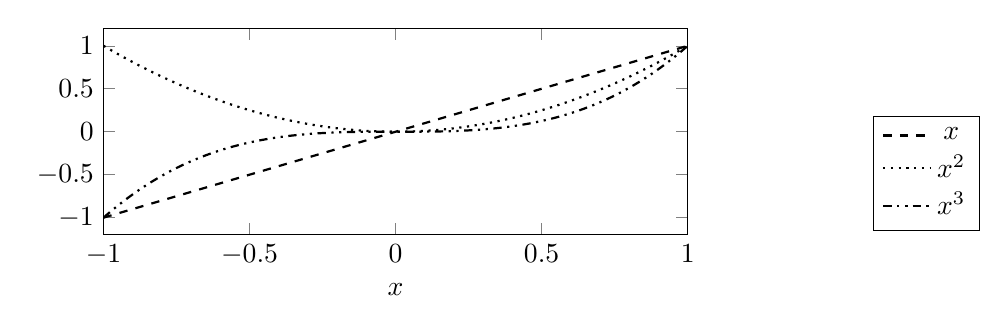
\begin{tikzpicture}
			\begin{axis}[
				width=9cm, height=4.2cm,
				domain=-1:1,
				samples=200,
				%axis lines*=left,        % removes bounding box, keeps left axis
				xlabel={$x$},
				ylabel={},
				ytick=\empty,
				ytick={-1,-0.5,0,0.5,1}, % manually set x-ticks
            			yticklabels={$-1$,$-0.5$,$0$,$0.5$,$1$},
				xtick={-1,-0.5,0,0.5,1}, % manually set x-ticks
            			xticklabels={$-1$,$-0.5$,$0$,$0.5$,$1$},
				xmin=-1, xmax=1,
				legend style={at={(1.5,0.02)},anchor=south east}
				]
				% f1 = x
				\addplot[thick, dashed] {x};
				\addlegendentry{$x$}
				% f2 = x^2
				\addplot[thick, dotted] {x^2};
				\addlegendentry{$x^{2}$}
				% f3 = x^3
				\addplot[thick, dashdotdotted] {x^3};
				\addlegendentry{$x^{3}$}
			\end{axis}
			\end{tikzpicture}
		\caption{The first few powers of an \gls{rv} $x$. The MGF 
		encodes the moments of $x$, which are the \glspl{expectation} 
		of the powers $x^{k}$ for $k=1,\,2,\,\ldots$.}
		\end{figure}
		The MGF is a useful tool for the study of sums of independent 
		\glspl{rv}. As a case in point, if $x$ and $y$ are independent 
		\glspl{rv}, then the MGF of their sum $z = x + y$ typically 
		satisfies $\mgf{z}{t} = \mgf{x}{t}\,\mgf{y}{t}$,
        		i.e., the MGF of the sum is typically the pointwise product of the 
		individual MGFs \cite[p.~280]{BillingsleyProbMeasure}.
		\\
 		See also: \gls{rv}, \gls{expectation}. }, 
 	first={moment generating function (MGF)}, 
 	firstplural={moment generating functions (MGFs)}, 
 	plural={MGFs}, 
 	type=math, 
 	text={MGF}
} 

\newglossaryentry{chernoffbound}
{name={Chernoff bound}, 
	description={TBC\index{Chernoff bound}.}, 
 	first={Chernoff bound}, 
 	type=math, 
 	text={Chernoff bound}
}

\newglossaryentry{rankdeficient}
{name={rank-deficient},
	description={A \gls{matrix} $\mA \in \mathbb{R}^{\samplesize \times \nrfeatures}$ 
         	is rank-deficient\index{rank-deficient} if it is not \gls{fullrank}, i.e., 
         	when $\rank{\mA} < \min\{\samplesize,\nrfeatures\}$.
 		\begin{figure}[H]
			\begin{center}
			\begin{tikzpicture}[x=2cm]
				% LEFT: Standard basis vectors and unit square
				\begin{scope}
					\draw[->, thick] (0,0) -- (1,0) node[below] {$\vu^{(1)}$};
					\draw[->, thick] (0,0) -- (0,1) node[above] {$\vu^{(2)}$};
					%\draw[fill=gray!15] (0,0) -- (1,0) -- (1,1) -- (0,1) -- cycle;
					%\node at (0.5,0.5) {\small unit square};
					%\node at (0.5,-0.6) {standard basis};
				\end{scope}
				% RIGHT: Transformed basis vectors and parallelogram
				\begin{scope}[shift={(3.2,0)}]
				%\draw[->, thick] (0,0) -- (1,0) node[below] {$\vv^{(1)}$};
				%	\draw[->, thick] (0,0) -- (0,1) node[above] {$\vv^{(2)}$};
					\coordinate (A) at (0.2,0.0);
					\coordinate (B) at (2.0,0.0);
					\draw[->, very thick, red] (0,0) -- (A) node[below,yshift=-2pt] {$\mA \vu^{(1)}$};
					\draw[->, very thick, red] (0,0) -- (B) node[above,yshift=2pt] {$\mA \vu^{(2)}$};
					%	\node[blue] at (0.25,1.25) {};
					%	\node at (0.8,-0.6) {transformed basis};
				\end{scope}
				% Arrow between plots
				\draw[->, thick] (1.6,0.5) to[bend left] node[midway, above] {$\mA$} (2.7,0.5);
				%	\draw[->, thick] (1.3,0.5) -- (2.4,0.5) node[midway, above] {$\mA$};
			\end{tikzpicture}
			\end{center}
		\caption{Example of a rank-deficient \gls{matrix} 
		$\mA \in \mathbb{R}^{2 \times 2}$.	\label{fig_matrix_rank_defdict}} 
		\end{figure} 
		In \gls{linreg}, the solution of the \gls{erm} problem is not 
		unique whenever the \gls{featuremtx} $\featuremtx$ is such that 
		the \gls{matrix} $\featuremtx^{\top}\featuremtx$ is rank-deficient.
		\\
   		See also: \gls{fullrank}, \gls{dimension}, \gls{vectorspace}. }, 
	first={rank-deficient}, 
   	type=math,
   	text={rank-deficient}
}

\newglossaryentry{fullrank}
 {name={full-rank},
 	description={A \gls{matrix} $\mA \in \mathbb{R}^{\samplesize \times \nrfeatures}$ 
  		is\index{full-rank} full-rank if it has \gls{maximum} \gls{rank} \cite{StrangLinAlg2016}. 
  		For a \gls{tallmatrix}, i.e., when $\nrfeatures < \samplesize$, being 
  		full-rank means that its \gls{rank} is equal to $\nrfeatures$. 
 		\begin{figure}[H]
			\centering
			\begin{tikzpicture}[every node/.style={font=\small}]
			% --- Full-rank square ---
			\node at (0,2) {$
			\mA =
			\begin{pmatrix}
			1 & 2\\
			3 & 4
			\end{pmatrix}
			$};
			\node[below=0.8cm of {$(0,2)$}] {\small full-rank square};
			% --- Rank-deficient square ---
			\node at (4.5,2) {$
			\mB =
			\begin{pmatrix}
			1 & 2\\
			2 & 4
			\end{pmatrix}
			$};
			\node[below=0.8cm of {$(4.5,2)$}] {\small \gls{rankdeficient} square};
			% --- Full-rank tall (3x2) ---
			\node at (0,-1.0) {$
			\mC =
			\begin{pmatrix}
			1 & 0\\
			0 & 1\\
			1 & 1
			\end{pmatrix}
			$};
			\node[below=1.2cm of {$(0,-1.0)$}] {\small full-rank \gls{tallmatrix}};
			% --- Rank-deficient wide (2x3) ---
			\node at (4.5,-1.0) {$
			\mD =
			\begin{pmatrix}
			1 & 2 & 3\\
			2 & 4 & 6
			\end{pmatrix}
			$};
			\node[below=1.2cm of {$(4.5,-1.0)$}] {\small \gls{rankdeficient} \gls{widematrix}};
			\end{tikzpicture}
		\caption{Examples of full-rank and \gls{rankdeficient} \glspl{matrix}.}
		\end{figure} 
  		A square \gls{matrix} is full-rank if and only if it is invertible. 
		\\ 
  		See also: \gls{matrix}, \gls{dimension}, \gls{linearmap}, \gls{columnspace}.}, 
	text = {full-rank}, 
  	type=math,
  	first={full-rank} 
 }

\newglossaryentry{rank}
{name={rank},
	description={The rank\index{rank} of a \gls{matrix} $\mA \in \mathbb{R}^{\samplesize \times \nrfeatures}$, 
 		denoted as $\rank{\mA}$, is the \gls{maximum} number of \gls{linearlyindep} columns 
 		of $\mA$ \cite{StrangLinAlg2016}. Equivalently, the rank can be defined as the 
 		\gls{dimension} of the \gls{columnspace} $\linspan{\mA} = \big\{ \mA \weights \mbox{ for some } 
 		\weights \in \mathbb{R}^{\nrfeatures} \big\}$. The rank of a \gls{matrix} 
 		$\mA \in \mathbb{R}^{\samplesize \times \nrfeatures}$ can neither exceed the 
 		number of rows nor the number of columns of $\mA$ \cite{Horn91}, \cite{MeyerMatrixAnalysis}, 
		i.e., $\rank{\mA} \leq \min \{ \samplesize, \nrfeatures \}$.  
		\\ 
 		See also: \gls{matrix}, \gls{dimension}, \gls{columnspace}, \gls{linearmap}.}, 
	text={rank}, 
	type=math,
	first={rank} 
}

\newglossaryentry{inverse}
{name={inverse matrix},
 description={An inverse \gls{matrix}\index{inverse matrix} $\mA^{-1}$ is defined for a 
 	square \gls{matrix} $\mA \in \mathbb{R}^{n \times n}$ that is of full rank, meaning its 
 	columns are linearly independent. In this case, $\mA$ is said to be invertible, 
 	and its inverse satisfies 
 	\[
 	\mA \mA^{-1} = \mA^{-1} \mA = \mI.
 	\]  	
     	A square \gls{matrix} is invertible if and only if its \gls{det} is non-zero. Inverse \glspl{matrix} are 
     	fundamental in solving systems of linear equations and in the closed-form solution of 
     	\gls{linreg} \cite{Strang2007}, \cite{Horn91}.  The concept of an inverse \gls{matrix} can be extended 
     	to \glspl{matrix} that are not square or does not have full \gls{rank}. One may define a ``left inverse'' $\mB$ 
     	satisfying $\mB \mA = \mI$ or a ``right inverse'' $\mC$ satisfying $\mA \mC = \mI$. 
     	For general rectangular or singular \glspl{matrix}, the Moore–Penrose \gls{pseudoinverse}
     	$\mA^{+}$ provides a unified concept of a generalized inverse \gls{matrix} \cite{GolubVanLoanBook}.
 	 \begin{figure}[H]
 		\centering
 		\begin{tikzpicture}[x=2cm,y=2cm]
 			% LEFT: Standard basis
 			\begin{scope}
 				\draw[->, thick] (0,0) -- (1,0) node[below right] {$\vx$};
 				\draw[->, thick] (0,0) -- (0,1) node[above left] {$\vy$};
 			\end{scope}
 			% CENTER: Transformed basis (by A)
 			\begin{scope}[shift={(2.0,0)}]
 				\coordinate (A) at (1.5,0.5);
 				\coordinate (B) at (-0.2,1.2);
				\draw[->, very thick, red] (0,0) -- (A) node[pos=0.5, below right] {$\mA \vx$};
 				\draw[->, very thick, red] (0,0) -- (B) node[above right] {$\mA \vy$};
 			\end{scope}
 			% RIGHT: Inverse transformation
 			\begin{scope}[shift={(4.9,0)}]
 				\draw[->, very thick, blue] (0,0) -- (1,0) node[pos=0.5, below] {$\mA^{-1} (\mA \vx) = \vx$};
 				\draw[->, very thick, blue] (0,0) -- (0,1) node[above] {$\mA^{-1} (\mA \vy) = \vy$};
 			\end{scope}
 			% Curved arrows between stages
 			\draw[->, thick, bend left=20] (1.2,0.4) to node[above] {$\mA$} (1.8,0.4);
 			\draw[->, thick, bend left=20] (3.8,0.4) to node[below] {$\mA^{-1}$} (4.4,0.4);
 		\end{tikzpicture}
 		\caption{A \gls{matrix} $\mathbf{A}$ represents a linear transformation of $\mathbb{R}^{2}$. The inverse \gls{matrix} $\mathbf{A}^{-1}$ 
 			represents the inverse transformation. \label{fig_matrix_inverse_dict}} 
 		\end{figure}
		See also: \gls{matrix}, \gls{det}, \gls{linreg}, \gls{pseudoinverse}.},
	first={inverse matrix},
		type=math,
	text={inverse matrix}
}

\newglossaryentry{matrix}
{name={matrix},
	description={A matrix\index{matrix} of size $\samplesize \times \nrfeatures$ is a 2-D array of numbers, 
 		which is denoted by 
		$$
  		\mA = \begin{pmatrix}
   		A_{1,1} & A_{1,2} & \dots  & A_{1,\nrfeatures} \\
		A_{2,1} & A_{2,2} & \dots  & A_{2,\nrfeatures} \\
		\vdots  & \vdots  & \ddots & \vdots \\
		A_{\samplesize,1} & A_{\samplesize,2} & \dots  & A_{\samplesize,\nrfeatures}
		\end{pmatrix} \in \mathbb{R}^{\samplesize \times \nrfeatures}.
		$$
		Here, $A_{\sampleidx,\featureidx}$ denotes the matrix entry in the $\sampleidx$th row and the 
		$\featureidx$th column. Matrices are useful representations of various mathematical objects \cite{StrangLinAlg2016},
		including the following:
		\begin{itemize}
			\item Systems of linear equations: We can use a matrix to represent a system of linear equations 
			$$ \begin{pmatrix}
			A_{1,1} & A_{1,2} \\
			A_{2,1} & A_{2,2}
			\end{pmatrix}
			\begin{pmatrix}
				w_1 \\
				w_2
			\end{pmatrix}
			=\begin{pmatrix}
				y_1 \\
				y_2
			\end{pmatrix}
			\quad \text{ compactly as } \quad \mA \vw = \vy.
			$$
    			One important example of systems of linear equations is the optimality condition for the 
    			\glspl{modelparam} within \gls{linreg}. 
			\item \Glspl{linearmap}:
			Consider a $\nrfeatures$-dimensional \gls{vectorspace} $\mathcal{U}$ and a $\samplesize$-dimensional \gls{vectorspace} $\mathcal{V}$. 
			If we fix a \gls{basis} $\mathbf{u}^{(1)},\,\ldots,\,\mathbf{u}^{(\nrfeatures)}$ for $\mathcal{U}$ and a \gls{basis} $\mathbf{v}^{(1)},\,\ldots,\,\mathbf{v}^{(\samplesize)}$ 
			for $\mathcal{V}$, each matrix $\mA \in \mathbb{R}^{\samplesize \times \nrfeatures}$ naturally defines a 
			\gls{linearmap} $\alpha: \mathcal{U} \rightarrow \mathcal{V}$ (see Fig. \ref{fig_matrix_dict}) such that
   			$$\vu^{(\featureidx)} \mapsto \sum_{\sampleidx=1}^{\samplesize} A_{\sampleidx,\featureidx} \vv^{(\sampleidx)}.$$
			\item \Glspl{dataset}: We can use a matrix to represent a \gls{dataset}. Each row 
			corresponds to a single \gls{datapoint}, and each column corresponds to a specific 
			\gls{feature} or \gls{label} of a \gls{datapoint}. 
		\end{itemize}
		\begin{figure}[H]
		\begin{center}
		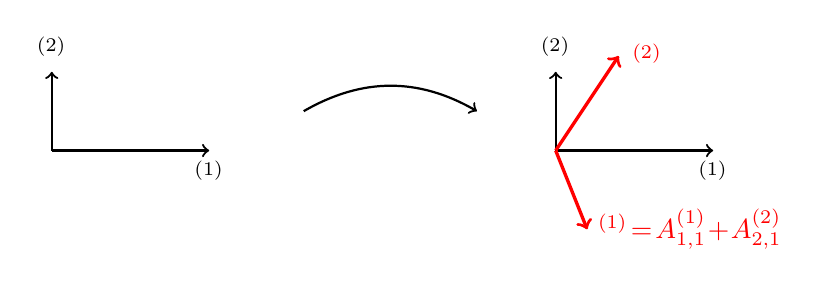
\begin{tikzpicture}[x=2cm]
			% LEFT: Standard basis vectors and unit square
			\begin{scope}
				\draw[->, thick] (0,0) -- (1,0) node[below] {$\vu^{(1)}$};
				\draw[->, thick] (0,0) -- (0,1) node[above] {$\vu^{(2)}$};
				%\draw[fill=gray!15] (0,0) -- (1,0) -- (1,1) -- (0,1) -- cycle;
				%\node at (0.5,0.5) {\small unit square};
				%\node at (0.5,-0.6) {standard basis};
			\end{scope}
			% RIGHT: Transformed basis vectors and parallelogram
			\begin{scope}[shift={(3.2,0)}]
				\draw[->, thick] (0,0) -- (1,0) node[below] {$\vv^{(1)}$};
				\draw[->, thick] (0,0) -- (0,1) node[above] {$\vv^{(2)}$};
				\coordinate (A) at (0.2,-1.0);
				\coordinate (B) at (0.4,1.2);
				\draw[->, very thick, red] (0,0) -- (A) node[below,right] {$\mA \vu^{(1)}\!=\!A_{1,1}\vv^{(1)}\!+\!A_{2,1}\vv^{(2)}$};
				\draw[->, very thick, red] (0,0) -- (B) node[right,xshift=1pt] {$\mA \vu^{(2)}$};
				%	\node[blue] at (0.25,1.25) {};
				%	\node at (0.8,-0.6) {transformed basis};
			\end{scope}
			% Arrow between plots
			\draw[->, thick] (1.6,0.5) to[bend left] node[midway, above] {$\mA$} (2.7,0.5);
		%	\draw[->, thick] (1.3,0.5) -- (2.4,0.5) node[midway, above] {$\mA$};
		\end{tikzpicture}
		\end{center}
		\caption{A matrix $\mA$ defines a \gls{linearmap} between two \glspl{vectorspace}. \label{fig_matrix_dict}} 
		\end{figure}
		See also: \gls{linearmap}, \gls{dataset}, \gls{linmodel}. },
	first={matrix},
	firstplural={matrices},
	type=math,
	plural={matrices},
	text={matrix}
}

\newglossaryentry{hyperplane}
{name={hyperplane},
	description={A hyperplane\index{hyperplane} is an $(\nrfeatures-1)$-dimensional affine 
				 subspace of a $\nrfeatures$-dimensional \gls{vectorspace}. In the 
				 context of an \gls{euclidspace} $\mathbb{R}^{\nrfeatures}$, a 
				 hyperplane is a set of the form
 				 \[ \{ \vx \in \mathbb{R}^\nrfeatures : \vw^\top \vx = b \},
  				 \]
                 where $\vw \in \mathbb{R}^d \setminus \{0\}$ is a normal \gls{vector} 
                 and $b \in \mathbb{R}$ is an offset. Such a hyperplane partitions 
				 $\mathbb{R}^\nrfeatures$ into two halfspaces
				\[\{ \vx \in \mathbb{R}^\nrfeatures : \vw^\top \vx \leq b \} \quad 
				\text{and} \quad \{ \vx \in \mathbb{R}^\nrfeatures : \vw^\top \vx \geq b \}.\]
 				Hyperplanes arise as the \glspl{decisionboundary} of \glspl{linclass}.},
	first={hyperplane},
	type=math,
	plural={hyperplanes}, 
	firstplural={hyperplanes},
	text={hyperplane}
}

\newglossaryentry{normalvector}
{name={normal vector},
	description={See\index{normal vector} \gls{hyperplane}.},
	first={normal vector},
	type=math,
	plural={normal vectors}, 
	firstplural={normal vectors},
	text={normal vector}
}

\newglossaryentry{halfspace}
{name={halfspace},
	description={See\index{halfspace} \gls{hyperplane}.},
	first={halfspace},
	type=math,
	plural={halfspaces}, 
	firstplural={halfspaces},
	text={halfspace}
}



\newglossaryentry{subspace}
{name={subspace},
	description={A subset of a \gls{vectorspace} $\mathcal{V}$ is a subspace\index{subspace} of $\mathcal{V}$ if it is also a 
		\gls{vectorspace} with respect to the same operations as $\mathcal{V}$.
			   \\
		See also: \gls{vectorspace}.},
	type=math, 
	first={subspace},
	text={subspace}
}

\newglossaryentry{columnspace}
{name={column space},
	description={The column space\index{column space} of a \gls{matrix} 
		$\mA \in \mathbb{R}^{\samplesize \times \nrfeatures}$,
		denoted by $\linspan{\mA}$, is the set of all linear combinations of the 
		columns of $\mA$. In other words, 
		$$ \linspan{\mA} = \{ \mA \weights : \weights \in \mathbb{R}^{\nrfeatures} \}. $$
		The column space $\linspan{\mA}$ of the \gls{matrix} $\mA$ 
		is a \gls{subspace} of the \gls{euclidspace} $\mathbb{R}^{\samplesize}$.
			   \\
		See also: \gls{matrix}, \gls{vectorspace}.},
	type=math,
	first={column space},
	text={column space}
}

\newglossaryentry{mvndist}
{name={multivariate normal distribution}, 
	description={The\index{multivariate normal distribution} multivariate normal distribution, 
		which is denoted by $\mvnormal{\meanvecgeneric}{\covmtxgeneric}$, is a fundamental 
		\gls{probmodel} for numerical \glspl{featurevec} of fixed dimension $\nrfeatures$. 
		It defines a family of \glspl{probdist} over \gls{vector}-valued \glspl{rv} 
		$\featurevec \in \mathbb{R}^{\nrfeatures}$~\cite{BertsekasProb}, \cite{GrayProbBook}, \cite{Lapidoth09}. 
		Each distribution in this family is fully specified by its \gls{mean} \gls{vector} 
		$\meanvecgeneric \in \mathbb{R}^{\nrfeatures}$ and \gls{covmtx} 
		$\covmtxgeneric \in \mathbb{R}^{\nrfeatures \times \nrfeatures}$. When the 
		\gls{covmtx} $\covmtxgeneric$ is invertible, the corresponding \gls{probdist} is 
		characterized by the following \gls{pdf}:
		\[p(\featurevec) = 
 		\frac{1}{\sqrt{(2\pi)^{\nrfeatures} \det\,(\covmtxgeneric)}} 
 		\exp\left[ -\frac{1}{2} 
 		(\featurevec - \meanvecgeneric)\,^{T}\, \covmtxgeneric^{-1} 
 		(\featurevec - \meanvecgeneric) \right].
 		\]
		Note that this \gls{pdf} is only defined when $\covmtxgeneric$ is invertible.
   		More generally, any \gls{rv} $\featurevec \sim \mvnormal{\meanvecgeneric}{\covmtxgeneric}$ 
   		admits the following representation:
  		\[
    		\featurevec = \mA \vz + \meanvecgeneric
   		\]
   		where $\vz \sim \mvnormal{\mathbf{0}}{\mathbf{I}}$ is a \gls{stdnormvec} 
   		and $\mA \in \mathbb{R}^{\nrfeatures \times \nrfeatures}$ satisfies $\mA \mA^\top = \covmtxgeneric$. 
   		This representation remains valid even when $\covmtxgeneric$ is singular, in which case $\mA$ 
   		is not full rank~\cite[Ch. 23]{Lapidoth2017}.
   		The family of multivariate normal distributions is exceptional among \glspl{probmodel} for numerical 
   		quantities, at least for the following reasons. First, the family is closed under affine 
   		transformations, i.e.,
		\[ 
		\featurevec \sim \mathcal{N}(\meanvecgeneric,\covmtxgeneric) \mbox{ implies } 
		\mB\featurevec\!+\!\vc \sim \mathcal{N}\big( \mB\meanvecgeneric+\vc,\mB \covmtxgeneric \mB\,^{T} \big). 
		\]
		Second, the \gls{probdist} $\mathcal{N}(\mathbf{0},\covmtxgeneric)$ maximizes the 
		\gls{diffentropy} among all distributions with the same \gls{covmtx} $\covmtxgeneric$~\cite{coverthomas}. 
		\\ 
		See also: \gls{probmodel}, \gls{probdist}, \gls{stdnormvec}, \gls{diffentropy}, \gls{gaussrv}.}, 
	first={multivariate normal distribution},
	type=math, 
	text={multivariate normal distribution}
}

\newglossaryentry{stdnormvec}
{name={standard normal random vector}, 
	description={A\index{standard normal vector} standard normal random \gls{vector} is a random 
		\gls{vector} $\vx=\big(x_{1}, \,\ldots, \,x_{\nrfeatures}\big)\,^{T}$ 
		whose entries are \gls{iid} \glspl{gaussrv} $x_{\featureidx} \sim \mathcal{N}(0,1)$. 
		It is a special case of a \gls{mvndist}, $\vx \sim \mathcal(\mathbf{0},\mathbf{I})$.
		\\ 
		See also: \gls{vector}, \gls{iid}, \gls{gaussrv}, \gls{mvndist}, \gls{rv}.}, 
	first={standard normal random vector},
	type=math, 
	text={standard normal random vector}
}